\section{Results}

\subsection{Baseline Model}

\subsection{Enhanced Model 1: UNet}
\begin{scriptsize}
	\vspace{-\parskip}
	\url{https://wandb.ai/mfixman-convolutional-team/work/runs/5ytrv216} \\[-4pt]
	\url{https://wandb.ai/mfixman-convolutional-team/work/runs/qbi7duzd}\footnotemark{}
	\footnotetext{The original run got preempted and was later continued; the section shows both runs together.}
\end{scriptsize}

While the UNet model has considerably better result than the baseline model, it overfits badly after only 15 epochs and doesn't learn much useful information afterwards.

\begin{figure}[h]
	\centering
	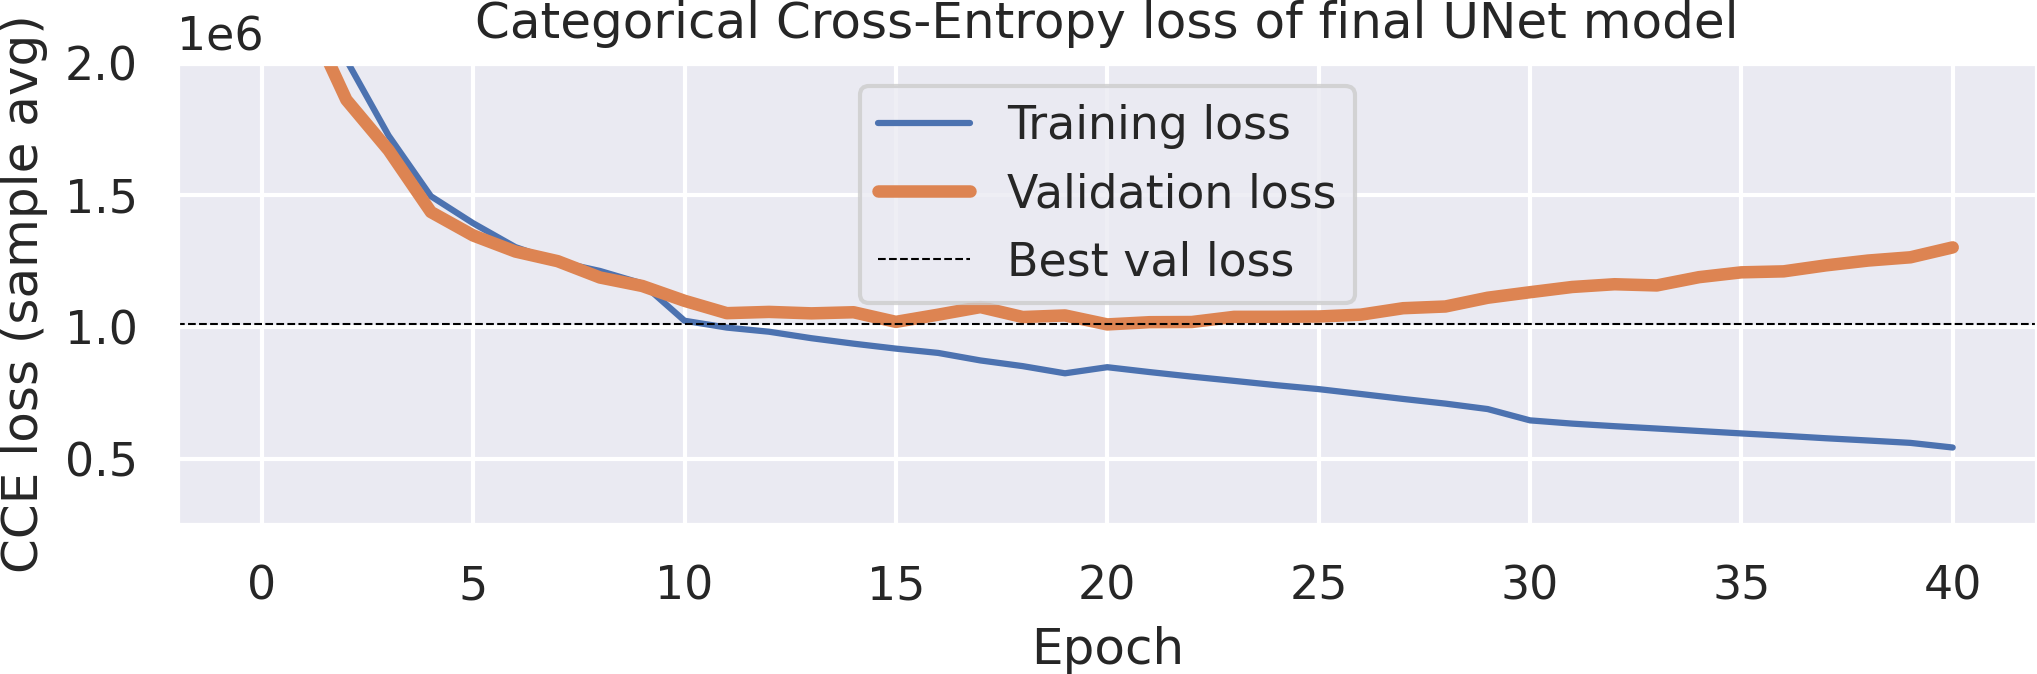
\includegraphics[width=.9\textwidth]{unet_loss.png}
	\caption{UNet model loss by epoch.}
\end{figure}

However, as seen in \cref{comparisons}, in practice it produces much better output than the baseline model.

\subsection{Enhanced Model 2: Swin2}
\begin{scriptsize}
	\vspace{-\parskip}
	\url{https://wandb.ai/mfixman-convolutional-team/work/runs/wspszqbr}
\end{scriptsize}

The Swin2 model has the lowest validation loss of the three models.
The dropout makes it overfit late and slowly; the best loss is found only after 30 epochs, and ever after overfitting the training loss drops slowly.

\begin{figure}[h]
	\centering
	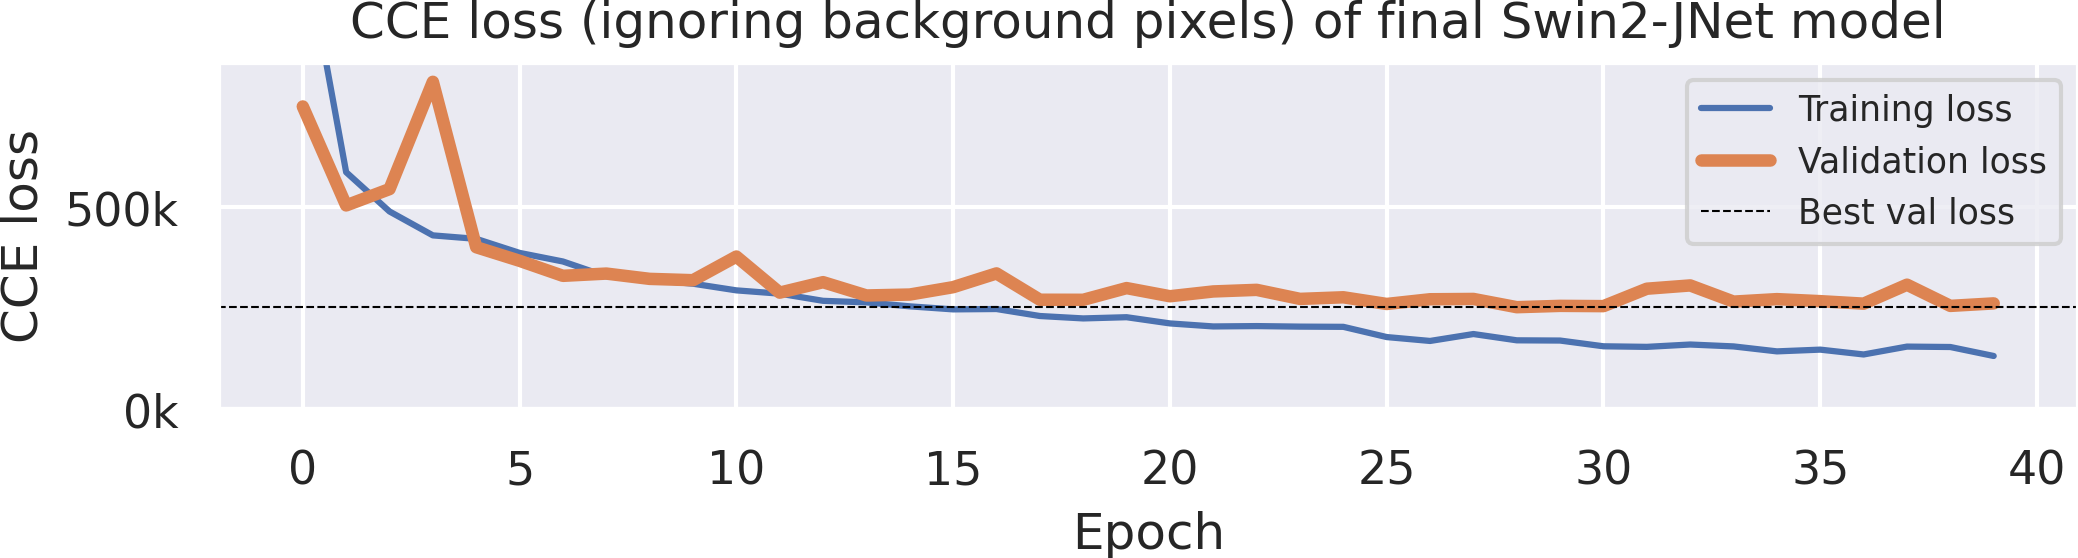
\includegraphics[width=.9\textwidth]{swin2_loss.png}
	\caption{Swin2-JNet loss by epoch.}
\end{figure}

The pre-trained weights in the transformer encoder seem to capture a lot of relevant picture information, which is later trained and used in the decoder.
This shows the promise of transfer learning: by only requiring to learn small but relevant details of the image, we can achieve a good loss in just a bit of training.

\subsection{Comparisons}
\label{comparisons}
